\section{Convex Optimization and Convex Analysis} % (fold)
\label{sec:convex_optimization_and_convex_analysis}

    In this section we cover a few topics which are related to convexity. Since we are considering (convex) optimization problems in this work we first want to define a convex program where we mainly follow \cite{Boyd}, whereas convex sets and convex functions are the basis of convex optimization.

    An optimization problem is of the form
        \begin{equation}
            \begin{array}{l l l}
                \min\limits_{u \in \mathbb{R}^{n}} & F(u) & \\
                \textnormal{subject to} & G_{i}(u) \le 0, & i = 1, ..., m \\
                & H_{j}(u) = 0 & j = 1, ..., p,
            \end{array}
            \label{eq:optimization_problem}
        \end{equation}
    where
        \begin{itemize}
            \item $u \in \mathbb{R}^{n}$ is called the \textit{optimization variable},
            \item $F: \mathbb{R}^{n} \longrightarrow \mathbb{R}$ \textit{objective function} or \textit{cost function},
            \item $G_{i}(u) \le 0$ \textit{inequality constraints} for all $i = 1, ..., m$,
            \item $H_{j}(u) = 0$ \textit{equality constraints} for all $j = 1, ..., p$,
            \item $G_{i}: \mathbb{R}^{n} \longrightarrow \mathbb{R}$ for all $i = 1, ..., m$ the \textit{inequality constraint functions} and
            \item $H_{j}(u) = 0$ for all $j = 1, ..., p$ the \textit{equality constraint functions}.
        \end{itemize}
    If we have no constraints, meaning $m = p = 0$, we say the problem \ref{eq:optimization_problem} is \textit{unconstrained}. It is called convex if all, the objectiv, equality and inequality functions, are convex.\\
    Further, we define the domain of the optimization problem \ref{eq:optimization_problem} by
        \begin{equation}
            \mathcal{D} = \textnormal{dom}(F) \cap \bigcap_{i = 1}^{m} \textnormal{dom}(G_{i}) \cap \bigcap_{j = 1}^{p} \textnormal{dom}(H_{j}).
            \label{eq:domain_of_optimization_problem}
        \end{equation}
    This set is the set of points for which the objective and all constraint functions are defined. We call a point $u \in \mathcal{D}$ \textit{feasible} if it satisfies all constraints. The optimization problem \ref{eq:optimization_problem} is said to be feasible if there exists at least one feasible point, and \textit{infeasible} otherwise. We call the set of all feasible points the \textit{feasible set} or alternatively the \textit{constraint set}.\\
    We define the optimal value $u^{\ast}$ of the problem \ref{eq:optimization_problem} by
        \begin{equation}
            u^{\ast} = \inf \big\{ F(u) : G_{i}(u) \le 0, i = 1, ..., m, H_{j}(u) = 0, j = 1, ..., p \big\},
        \end{equation}
    where we allow $u^{\ast}$ to take on the extended values $\pm \infty$. We set $u^{\ast} = \infty$ if the problem is infeasible, since $\inf(\emptyset) = \infty$. If there are feasible points $u_{k}$ with $F(u_{k}) \longrightarrow -\infty$ as $k \longrightarrow \infty$, then $u^{\ast} = -\infty$, and we say that problem \ref{eq:optimization_problem} is \textit{unbounded below}.\\

    Since, convex optimization is based on convex functions we need to define these class of functions and its properties.
    According to \cite{Chambolle-et-al-10} we have the following basic definitions, propositions and theorems.

    \begin{definition}[Convex Set] % (fold)
    \label{def:convex_set}

        A subset $C \subseteq X$ is said to be convex if and only if for any $u_{1}, u_{2} \in C$, the line segment $[u_{1}, u_{2}] \subseteq C$, that is, for any $t \in [0, 1]$,
            \begin{equation}
                u_{1}t + u_{2}(1 - t) \in C.
                \label{eq:convex_set}
            \end{equation}
        We call $C$ strictly convex, if it is closed and
            \begin{equation}
                (1 - t)u_{1} + u_{2}t \in \textnormal{int}\,C, \,\,\, \forall u_{1}, u_{2} \in C, \,\,\, u_{1} \ne u_{2}, \,\,\, t \in [0, 1],
                \label{eq:strictly_convex_set}
            \end{equation}
        where \textnormal{int} stands for interior.

    \end{definition}
    % definition convex_set (end)

    This definition ensures that if $C$ is convex, we can always find two arbitrary points in $C$ such that the line segment $[u_{1}, u_{2}]$ with end points $u_{1}, u_{2}$ lies fully in $C$ (see Figure \ref{fig:convex_and_non_convex_sets}).
    \begin{figure}[ht]
        \centering
        \begin{subfigure}[b]{0.3\textwidth}
            
\includegraphics[width=\textwidth]{img/unit_l1_norm.png}
            \caption{$l_{1}$ unit sphere}
            \label{fig:unit_l2_norm}
        \end{subfigure}
        \begin{subfigure}[b]{0.3\textwidth}
            
\includegraphics[width=\textwidth]{img/unit_l2_norm.png}
            \caption{$l_{2}$ unit sphere}
            \label{fig:unit_l1_norm}
        \end{subfigure}
        \begin{subfigure}[b]{0.3\textwidth}
            
\includegraphics[width=\textwidth]{img/non_convex_set.png}
            \caption{Star: a non-convex set.}
            \label{fig:star}
        \end{subfigure}
        \caption{We see three different sets, where (a) and (b) are convex, but (c) is not. (a) refers to the unit sphere of the $l_{1}$ norm where (b) refers to the unit sphere of the $l_{2}$ norm. In (c) we see that the line segment of $[u_{2}, u_{3}]$ lies not in the set itself.}
        \label{fig:convex_and_non_convex_sets}
    \end{figure}

    \begin{definition}[Inidcator Function, Support Function] % (fold)
    \label{def:indicator_function}

        For any subset $C \subseteq X$ of a vector space, the indicator function $\delta_{C}: X \longrightarrow \mathbb{R}_{\infty}$ is defined as
            \begin{equation}
                \delta_{C}(u) =
                \left\{
                    \begin{array}{l l}
                      0      & \quad \text{if $u \in C$}, \\
                      \infty & \quad \text{if $u \notin C$}.
                    \end{array}
                \right.
            \label{eq:indicator_function}
            \end{equation}
        The support function of the set $C$ is defined as
            \begin{equation}
                S_{C}(u) = \sup_{p \in C} \langle p, u \rangle,
            \label{eq:support_function}
            \end{equation}
        where we allow $S_{C}(u)$ to be $+\infty$.

    \end{definition}
    % definition indicator_function (end)

    \begin{definition}[Convex Function, Proper, Lower-Semicontinuouity] % (fold)
    \label{def:convex_function_proper_lower_semicontinuous}

        A function $F: X \longrightarrow \mathbb{R}_{\infty}$ is said to be
            \begin{itemize}
                \item convex if for all $u_{1}, u_{2} \in C$ and any $t \in [0, 1]$ the inequality
                \begin{equation}
                    F(u_{1}t + u_{2}(1 - t)) \le F(u_{1})t + F(u_{2})(1 - t)
                    \label{eq:convex_function}
                \end{equation}
                is satisfied. $F$ is called strictly convex, if the inequality \ref{eq:convex_function} holds strictly whenever $u_{1}, u_{2}$ are distinct points and $t \in (0, 1)$.
                \item proper if $F$ is not identically $-\infty$ or $+\infty$.
                \item lower-semicontinuous (l.s.c) if for any $u \in X$ and a sequence $(u_{n})$ converging to $u$,
                    \begin{equation}
                        F(u) \le \liminf_{n \rightarrow \infty} F(u_{n}).
                        \label{eq:lower_semicontinuous}
                    \end{equation}
            \end{itemize}
        We define $\Gamma_{0}(X)$ as the set of all convex, proper, l.s.c. functions on $X$.

    \end{definition}
    % definition convex_function_proper_lower_semicontinuous (end)

    A common example for a strictly convex function would be a quadratic function (see Example \ref{ex:convex_function}). In Figure \ref{fig:convex_function} (a) this is also illustrated, together with the plot in (b) of the function
        \begin{equation}
            F(u) =
                \begin{dcases*}
                    u^{2} & \textnormal{$x \in [-1, 1]$} \\
                    - \frac{1}{2} u(u - 4) & \textnormal{$x \in (1, 3]$}.
                \end{dcases*}
            \label{eq:lsc_example}
        \end{equation}
    being lower-semicontinuous.

    \begin{proposition} % (fold)
        
        Let $F, G: X \longrightarrow \mathbb{R}_{\infty}$ be two convex functions. Then $F + G$ is also convex.

    \end{proposition}
    % proposition (end)

    \begin{proof} % (fold)
        This can easily be verified. Define $H(u) = F(u) + G(u)$ with $F, G$ convex and choose $u_{1}, u_{2} \in X$ and $t \in [0, 1]$, then we obtain
        \begin{eqnarray}
            H(u_{1}t + u_{2}(1 - t)) &=& F(u_{1}t + u_{2}(1 - t)) + G(u_{1}t + u_{2}(1 - t)) \notag \\ 
            &\le& F(u_{1})t + F(u_{2})(1 - t) + G(u_{1})t + G(u_{2})(1 - t) \notag \\
            &=& \underbrace{F(u_{1})t + G(u_{1})t}_{= H(u_{1})t} + \underbrace{F(u_{2})(1 - t) + G(u_{2})(1 - t)}_{H(u_{2})(1 - t)} \notag \\
            &=& H(u_{1})t + H(u_{2})(1 - t), \notag
        \end{eqnarray}
        which shows that $H$ is convex.\qed
    \end{proof}
    % proof (end)

    \begin{remark}[Concave Function] % (fold)
        \label{rem:concave_function}

        Let $F$ be as in Definition \ref{def:convex_function_proper_lower_semicontinuous}. If $-F$ is (strictly) convex, then we say that $F$ is (strictly) concave. If $F$ is both convex and concave we say that $F$ is affine, i.e. equality holds in Equation \ref{eq:convex_function}.

    \end{remark}
    % remark concave_function (end)

    \begin{figure}[ht]
        \centering
        \begin{subfigure}[b]{0.4\textwidth}
        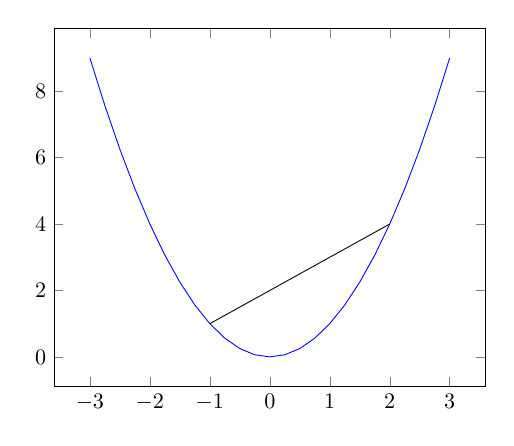
\begin{tikzpicture}[scale=0.8]
            \begin{axis}
                \addplot[domain=-3:3,blue] {x*x};
                \addplot[domain=-1:2,black] {x + 2};
            \end{axis}
        \end{tikzpicture}
        \caption{A quadratic function.}
        \end{subfigure}
        \begin{subfigure}[b]{0.4\textwidth}
        \begin{tikzpicture}[scale=0.8]
            \begin{axis}
                \addplot[domain=-1:1,blue] {x*x};
                \addplot[domain=1:3,blue] {-0.5*x*(x-4)};
                \draw[dotted] (axis cs:1,-1) -- (axis cs:1,3);
                \addplot[soldot] coordinates{(1,1)};
                \addplot[holdot] coordinates{(1,1.5)};
            \end{axis}
        \end{tikzpicture}
        \caption{A l.s.c. function.}
        \end{subfigure}
        \caption{(a) shows one line segment above a convex (quadratic) function which lies completely in $\textnormal{epi}(F)$. (b) is the l.s.c. function of Equation \ref{eq:lsc_example}. The left part of the plots accesses the value at $(1, 1)$, but the right part does not.}
        \label{fig:convex_function}
    \end{figure}

    \begin{example} % (fold)
    \label{ex:convex_function}

        \begin{enumerate}
            \item Let $A \in \mathbb{R}^{m \times n}$ be a real matrix and $F: \mathbb{R}^{n} \longrightarrow \mathbb{R}^{m}$ a linear function with $F(u) = Au$. Then $F$ is convex and concave, hence linear functions are affine.
                \begin{proof} % (fold)
                    Choose $u_{1}, u_{2} \in \mathbb{R}, t \in [0, 1]$. We get
                    $$
                       F(u_{1}t + u_{2}(1 - t)) = F(u_{1}t) + F(u_{2}(1 - t)) = F(u_{1})t + F(u_{2})(1 - t)
                    $$
                    by definition of linearity.\qed
                \end{proof}
                % proof (end)
            \item Let $A \in \mathbb{R}^{n \times n}$ be a real, symmetric, positiv definite matrix and $F: \mathbb{R}^{n} \longrightarrow \mathbb{R}^{n}$ a linear function with $F(u) = \frac{1}{2}u^{T}Au + b^{T}u + c$. Then $F$ is strictly convex. To show this we make use of a fundamental result of the calculus class. Since, if $\mathcal{H}\big(F(u)\big) > 0$ then the function $F$ is strictly convex. Here $\mathcal{H}$ stands for the Hessian of the function $F$. We have
                $$
                    \mathcal{H}\big(F(u)\big) = A > 0
                $$
            by definition.
            \item This example will later be useful: Each norm $||\cdot||: X \longrightarrow \mathbb{R}$ on a normed vector space $X$ is convex (see also Figure \ref{def:convex_function_proper_lower_semicontinuous}).
                \begin{proof} % (fold)
                    Choose $u, v \in X, t \in [0, 1]$, then
                    $$
                        ||ut + v(1 - t)||_{X} \overbrace{\le}^{(\ast)} ||ut||_{X} + ||v(1 - t)||_{X} \overbrace{=}^{(\ast\ast)} ||u||_{X} t + ||v||_{X} (1 - t).
                    $$
                    In $(\ast)$ we used the triangle inequality and in $(\ast\ast)$ absolute homogeneity with the fact that $t \in [0, 1]$.\qed
                \end{proof}
                % proof (end)
        \end{enumerate}

    \end{example}
    % example convex_function (end)

    Sometimes in literature you find another definition of convex functions. Therefore let us first introduce the epigraph and the domain of a function.

    \begin{definition}[Domain, Epigraph] % (fold)
    \label{def:domain_epigraph}

        For any function $F: X \longrightarrow \mathbb{R}_{\infty}$, we define the domain
            \begin{equation}
                \textnormal{dom}(F) = \{ u \in X : F(u) < +\infty \},
                \label{eq:domain}
            \end{equation}
        and the epigraph
            \begin{equation}
                \textnormal{epi}(F) = \{ (u, t) \in X \times \mathbb{R}: t \ge F(u) \} \in \mathbb{R}^{n+1}.
                \label{eq:epigraph}
            \end{equation}
    \end{definition}
    % definition domain_epigraph (end)

    Then we have the following definition for a convex function.

    \begin{definition}[Convex Function] % (fold)
    \label{def:convex_function_else}

        A function $F: X \longrightarrow \mathbb{R}_{\infty}$ is convex if $\textnormal{dom}(F)$ and $\textnormal{epi}(F)$ are convex sets.

    \end{definition}
    % definition convex_function_else (end)

    \begin{definition}[Closed Function] % (fold)
    \label{def:closed_function}

        Let $F: X \longrightarrow \mathbb{R}_{\infty}$ be a function. Then $F$ is closed if $\textnormal{epi}(F)$ is a closed set.

    \end{definition}
    % definition closed_function (end)

    \begin{figure}[ht]
        \centering
        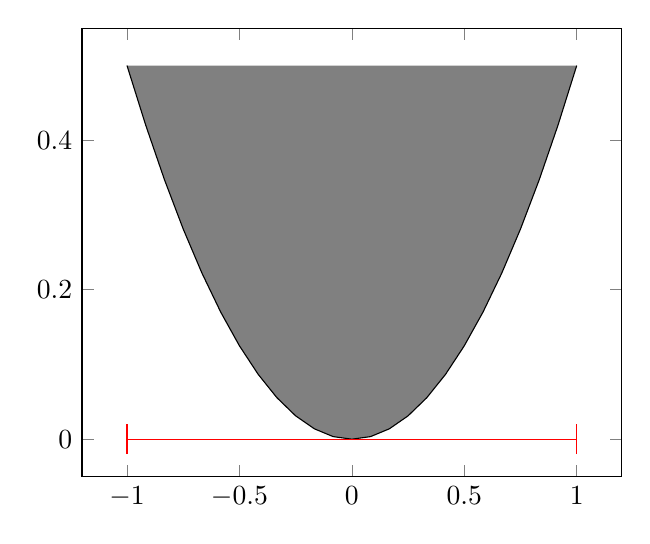
\begin{tikzpicture}
            \begin{axis}
                \addplot[domain=-1:1,black,fill=gray] {0.5*x*x};
                \draw[red] (axis cs:-1,0) -- (axis cs:1,0);
                \draw[red] (axis cs:-1,-0.02) -- (axis cs:-1,0.02);
                \draw[red] (axis cs:1,-0.02) -- (axis cs:1,0.02);
            \end{axis}
        \end{tikzpicture}
        \label{fig:domain_epigraph}
        \caption{Domain (red), denoted as $\textnormal{dom}(F) = [-1, 1]$ and epigraph \\$\textnormal{epi}(F) = \{(u, t) \in [-1, 1] \times \mathbb{R} : t \ge \frac{1}{2}u^{2}\}$ (gray) of a function $F: [-1, 1] \longrightarrow \mathbb{R}$ with $F(u) = \frac{1}{2}u^{2}$.}
    \end{figure}

    Now, that we are set up with convexity, we want to introduce one of the most important concepts for this thesis.

    \begin{definition}[Legendre-Fenchel conjugate] % (fold)
    \label{def:legendre_fenchel_conjugate}

        Let $F: X \longrightarrow \mathbb{R}_{\infty}$ be a convex function. We define the Legendre-Fenchel conjugate $F^{\ast}$ of $F$ for any $p \in X$ by
            \begin{equation}
                F^{\ast}(p) = \sup_{u \in X} \big( \langle p, u \rangle - F(u) \big).
                \label{eq:legendre_fenchel_conjugate}
            \end{equation}

    \end{definition}
    % definition legendre_fenchel_conjugate (end)

    \begin{remark} % (fold)
        Without a proof we state that $F^{\ast}$ - as the supremum of linear, continuous functions - is convex and lower-semicontinous, even $F$ is not. In addition $F^{\ast}$ is proper if $F$ is convex and proper.
    \end{remark}
    % remark (end)

    \begin{theorem} % (fold)
        Let $F \in \Gamma_{0}(X)$, then $F^{\ast\ast} = F$.
    \end{theorem}
    % theorem (end)

    The last theorem assures that we can rewrite Equation \ref{eq:legendre_fenchel_conjugate} to derive
        $$
            F(u) = \big( F^{\ast}(p) \big)^{\ast}(u) = \sup_{p \in Y} \big( \langle u, p \rangle - F^{\ast}(p) \big).
        $$
    \begin{example}
    \label{ex:legendre_fenchel_conjugate_example}

        Let us view some examples on the Legendre-Fenchel conjugate.
        \begin{enumerate}
            \item The Legendre-Fenchel conjugate of the indicator function of a set $C \subseteq X$ is given by
                $$
                    \delta^{\ast}_{C}(p) = \sup_{u \in C} \langle p, u \rangle - \delta_{C}(u) = \sup_{u \in C} \langle p, u \rangle,
                $$
            which is the support function.
            \item Let $F$ be an arbitrary function in $X$ and $\alpha > 0$. Then the convex conjugate of $\alpha F(u)$ is given by
                $$
                    F^{\ast}(p) = \alpha F^{\ast}(\frac{p}{\alpha}).
                $$
            To show this we just compute
                $$
                    F^{\ast}(p) = \sup_{u \in X} \langle p, u \rangle - \alpha F(u) = \alpha \big( \underbrace{\sup_{u \in X} \langle \frac{p}{\alpha}, u \rangle - F(u)}_{= F^{\ast}(\frac{p}{\alpha})} \big) = \alpha F^{\ast}(\frac{p}{\alpha}).
                $$
            \item Now, let $||\cdot||$ be a norm on $X$, with dual norm $||\cdot||_{\ast}$ on $Y$. We show that
                $$
                    F^{\ast}(p) =
                        \begin{dcases*}
                            0 & \textnormal{if $||p||_{\ast} \le 1$,} \\
                            \infty & \textnormal{else},
                        \end{dcases*}
                $$
            i.e. the conjugate of a norm is the indicator function of the dual norm unit ball. We have
                $$
                    F^{\ast}(p) = \sup_{u \in X} (\langle p, u \rangle - ||u||).
                $$
            First let $||p||_{\ast} > 1$. By definition of the dual norm ($||p||_{\ast} = \sup\limits_{||x|| \le 1} |p^{T}x|$) there is a $x \in \mathbb{R}^{n}$ and we observe $p^{T}x > 1$.

            We take $u = tx$ and let $t \longrightarrow \infty$, then we get
                $$
                    \langle p, u \rangle - ||u|| = t(\langle p, z \rangle - ||z||) \longrightarrow \infty,
                $$
            which shows that $F^{\ast}(p) = \infty$. On the other hand if $||p||_{\ast} \le 1$ we have
                $$
                    \langle p, u \rangle \le ||u|| \, ||p||_{\ast}
                $$
            for all $u \in X$. But this implies
                $$
                    \langle p, u \rangle - ||u|| \le ||u|| \, ||p||_{\ast} - ||u|| = ||u|| \, (||p||_{\ast} - 1) \le 0.
                $$
            To get the supremum we need to choose $u = 0$ which shows that $F^{\ast} = 0$ for this case.
            \item As a last example we show that for a function $F(u) := \frac{1}{2} ||u||^{2}$ its conjugate is $F^{\ast}(p) = \frac{1}{2} ||p||_{\ast}^{2}$. With Cauchy-Schwarz-inequality we know that $\langle p, u \rangle \le ||p||_{\ast}\,||u||$. We observe
                $$
                    \langle p, u \rangle - \frac{||u||^{2}}{2} \le ||p||_{\ast}\,||u|| - \frac{||u||^{2}}{2},
                $$
            where the righthand side is a quadratic function of $||u||$. Define $H(x) := -\frac{x^{2}}{2} + y\,x$, then clearly the maximal value of $H$ is $x = y$. Plugging $||u||$ into $H$ we see, that the maximum is attained at $||p||_{\ast}$. It follows
                $$
                    \langle p, u \rangle - \frac{||u||^{2}}{2} \le \frac{||p||_{\ast}^{2}}{2}.
                $$
            This shows that $F^{\ast}(p) \le \frac{||p||_{\ast}^{2}}{2}$. Let us now proof the inequality in the other direction. We assume that we find an arbitrary $u$ which satisfies $\langle u, p \rangle = ||u||\,||p||_{\ast}$. Further, we assume that $||u|| = ||p||_{\ast}$ where $u$ is scaled so that the last equation holds. Then we have
                $$
                    \langle p, u \rangle - \frac{||u||^{2}}{2} = ||u||\,||p||_{\ast} - \frac{||u||^{2}}{2} = \frac{||p||^{2}_{\ast}}{2},
                $$
            but for this particular $u$ it holds that
                $$
                    \langle p, u \rangle - \frac{||u||^{2}}{2} \le \sup\limits_{u \in X} \langle p, u \rangle - \frac{||u||^{2}}{2} = F^{\ast}(p).
                $$
            From these two inequalities it follows that $F^{\ast}(p) = \frac{||p||_{\ast}^{2}}{2}$
        \end{enumerate}
    \end{example}

    Another important property of functions is differentiability. Unfortunatelly, in some cases a function $F$ is not differentiable everywhere. For this, we want to define the so called subdifferential and therefore the subgradient.

    \begin{definition}[Subgradient, Subdifferential] % (fold)
        \label{def:subgradient_subdifferential}

        Let $X$ be an open, convex set and $F: X \longrightarrow \mathbb{R}_{\infty}$ a (convex) function. A vector $p$ is called subgradient of $F$ in $u_{0} \in X$, if
            \begin{equation}
                F(u) \ge F(u_{0}) + \langle p, u - u_{0} \rangle \,\,\, \forall u \in X. \label{eq:subgradient}
            \end{equation}
        The set
            \begin{equation}
                \partial F(u_{0}) = \{ p \in X: \, F(u) \ge F(u_{0}) + \langle p, u - u_{0} \rangle \,\,\, \forall u \in \textnormal{dom}(F) \}
            \end{equation}
        is called subdifferential of $F$ in $u_{0} \in X$ and $\textnormal{dom}(\partial F) = \{ u: \partial F(u) \ne \emptyset \} \subset F$.

    \end{definition}
    % definition subgradient_subdifferential (end)

    If $F$ and $G$ are differentiable we have $\partial(F + G) = \partial F + \partial G$. For the subdifferential this holds under some conditions. We want to give the corresponding Proposition without giving a proof. We just state that in our computations this equality can always be used.

    \begin{proposition} % (fold)

        Let $F, G$ be convex and assume $\textnormal{int} (\textnormal{dom} G) \cap \textnormal{dom} F \ne \emptyset$: then
            $$
                \partial(F + G) = \partial F + \partial G.
            $$
    
    \end{proposition}
    % proposition (end)

    To illustrate the subgradient and subdifferential, respectively, we want to give some examples.

    \begin{example}
    \label{ex:subgradient_subdifferential}

        \begin{enumerate}
            \item Take the absolute value function $F(u) = |u|$ in $\mathbb{R}$ which is defined by
                $$
                    F(u) =
                        \begin{dcases*}
                            u & \textnormal{if $u \ge 0$,} \\
                            -u & \textnormal{else}.
                        \end{dcases*}
                $$
            Since $F(u)$ is not differentiable in $0$, but on $\mathbb{R} / \{0\}$ we compute the subgradient as
                \begin{itemize}
                    \item $\partial F(u) = 1$ if $u > 0$,
                    \item $\partial F(u) = -1$ if $u < 0$,
                    \item and finally
                        $$
                            F(0) + p(u - 0) \le F(u) \Longleftrightarrow p \cdot u \le |u|.
                        $$
                    If $u \ge 0$ this is equivalent to $p \ge 1$. If $u < 0$ we get
                        $$
                            p \cdot u \le |u| \Longleftrightarrow p \cdot u \le -u \Longleftrightarrow p \ge -1.
                        $$
                \end{itemize}
            Finally, we have
                $$
                    p =
                        \begin{dcases*}
                            1 & \textnormal{if $u > 0$,} \\
                            -1 & \textnormal{if $u < 0$,} \\
                            [-1, 1] & \textnormal{if $u = 0$.}
                        \end{dcases*}
                $$
            \item Let $F(u) = ||u||_{1}$. As a non-differentiable convex function we seek for the subdifferential. For that we can express the $l_{1}$-norm as 
                $$
                    ||u||_{1} = |u_{1}| + ... + |u_{n}| = \max \big\{ p^{T}u : p_{i} \in \{-1, 1\} \big\},
                $$
             for all $u \in X$. Obviously, one gets $||p||_{\infty} \le 1$. %This would solve the inequality \ref{eq:subgradient}
             If we find a $p$ such that $p^{T}u = ||u||_{1}$ then immediately inequality \ref{eq:subgradient} would be satisfied, because
                $$
                    F(u) \ge F(u_{0}) + p^{T} u \Longleftrightarrow ||u||_{1} \ge 0 + p^{T} u = ||u||_{1}.
                $$
            On the other hand, if we choose $p_{i} = -1$ if $u_{i} < 0$ and $p_{i} = 1$ if $u_{i} > 0$ (this was also what we got by calculating the subgradient of the absolute value function) we only have the case left where $u_{i} = 0$. In this case, we can choose both $p_{i} = -1$ or $p_{i} = 1$ or equivalently looking at the non-differentiable point $u_{0} = 0$ and if $||p||_{\infty} \le 1$, we observe
                $$
                    F(u) \ge F(0) + p^{T} (u - 0) \Longleftrightarrow ||u||_{1} \ge p^{T}u.
                $$
            This means we have
                $$
                    p =
                        \begin{dcases*}
                            1 & \textnormal{if $u > 0$,} \\
                            -1 & \textnormal{if $u < 0$,} \\
                            -1 \,\textnormal{or}\, 1 & \textnormal{if $u = 0$.}
                        \end{dcases*}
                $$
            and
                \begin{equation}
                    \partial F(u) = \big\{ p : ||p||_{\infty} \le 1, \, p^{T}u = ||x||_{1} \big\}.
                    \label{eq:subdifferential_of_l1_norm}
                \end{equation}
        \end{enumerate}
    \end{example}

    The following Propositions are elementary for computations later. We provide them without giving a proof and refer to \cite{Rockafellar} and \cite{Chambolle-et-al-10}.

    \begin{proposition} % (fold)

        Let $F \in \Gamma_{0}(X)$. Then

        \begin{itemize}
            \item the set of minimizers $\arg \min\limits_{u \in X} F(u)$ is convex (possibly empty).
            \item if $\hat{u}$ is a local minimum of $F$, then $\hat{u}$ is in fact a global minimum, i.e.
                $$
                    \hat{u} \in \arg \min_{u \in X} F(u).
                $$
        \end{itemize}

    \end{proposition}
    % proposition (end)

    \begin{proposition} % (fold)
    \label{prop:convex_subgradient}
        
        For any $F$ convex, $p \in \partial F(u)$ if and only if

            $$
                \langle p, u \rangle - F(u) = F^{\ast}(p).
            $$

        Moreover if $F \in \Gamma_{0}$, so that $F^{\ast\ast} = F$, then this is equivalent to $u \in \partial F^{\ast}(p)$.

    \end{proposition}
    % proposition convex_subgradient (end)

    \begin{proposition} % (fold)
    \label{prop:zero_element_of_subgradient}
        
        Let $F$ be convex, then $\hat{u} \in \arg \min\limits_{u \in X} F(u)$ if and only if $0 \in \partial F(\hat{u})$.

    \end{proposition}
    % proposition zero_element_of_subgradient (end)

    The three propositions from above are fundamental for our work. If we find a (local) minimizer of a convex optimization problem, we already know that this minimizer is the global optimum. Further, we see in Propositions \ref{prop:convex_subgradient} how the variables $u$ and $p$ can be interchanged by dealing with the subdifferential. The last statement assures, that if we find a global minimum of our convex optimization problem, then we have that $0$ always is an element of the subdifferential.\\ 
    The last theorem, we will provide, can be found in \cite{Rockafellar} and is used extensively in the following chapters. One can find different editions of the theorem, see for instance (yaoling paper). We provide it without a proof, for which we also refer to \cite{Rockafellar}. But, first we need:

    \begin{definition}[Projection Operator, Proximity Operator, Moreau Envelop] % (fold)
    \label{def:projection_operator}

        For any non-empty closed set $C$ the projection operator for an arbitrary point $z \notin C$ on the set $C$ is defined by
            \begin{equation}
                P_{l_{C}}(z) = \arg \min_{u \in C} \frac{1}{2} ||z - u||_{2}^{2},
                \label{eq:projection_operator}
            \end{equation}
        meaning the orthogonal projection onto the convex set $C$. We define the Proximity Operator in a similar fashion due to
            \begin{equation}
                \textnormal{prox}^{\alpha}_{F}(z) = \arg \min_{u \in X} \frac{1}{2} ||u - z||_{2}^{2} + \alpha \, F(u),
                \label{eq:proximity_operator}
            \end{equation}
        and the Moreau envelop as
            \begin{equation}
                M^{\alpha}_{F}(z) = \min_{u \in X} \frac{1}{2} ||u - z||_{2}^{2} + \alpha \, F(u),
                \label{eq:envelop_operator}
            \end{equation}
        for any $\alpha > 0$.
    \end{definition}
    % definition projection_operator (end)

    The Proximity operator is a strict generalization of the Projection operator, while the Moreau envelop is a generalization of the squared distance measure function. Later, we will work out the connection between the projection and the proximity operator in detail. Let us shortly view two useful examples for the projection operator.

    \begin{example}
    \label{ex:projection_operator}

        The $l_{p}$-Projection of a point $p \in \mathbb{R}^{n}$ onto the $l_{p}$-unit sphere with $p \notin C = \{u : ||u||_{p} \le 1 \}$ is given by the following minimization problem:
            \begin{equation}
                \begin{array}{l l}
                    \min\limits_{u \in C} &  \frac{1}{2} ||u - p||_{2}^{2} \\
                    \textnormal{subject to} & ||u||_{p} \le 1.
                \end{array}
            \end{equation}
        We are looking at the $l_{2}$-Projection (euclidean projection) and the $l_{\infty}$-Projection, where both convex optimization problems have unique solutions, for more information see for instance \cite{Jitkomut Songsiri}.
        \begin{enumerate}
            \item The solution for the euclidean projection is given by
                \begin{equation}
                    u^{\ast} =
                    \left\{
                        \begin{array}{l l}
                           p, & \textnormal{if}\,\, ||p||_{2} \le 1 \\
                           \frac{p}{||p||_{2}}, & \textnormal{otherwise.}
                        \end{array}
                    \right.
                \end{equation}
            Or equivalently one gets $P_{l_{2}}(u) = \frac{u}{\max(1, |u|)}$.
            \item For the $l_{\infty}$-Projection we observe
                \begin{equation}
                    u_{k}^{\ast} =
                    \left\{
                        \begin{array}{l l}
                           p_{k}, & \textnormal{if}\,\, |p_{k}| \le 1 \\
                           1, & \textnormal{otherwise,}
                        \end{array}
                    \right.
                \end{equation}
            for $k = 1, ..., n$ or $P_{l_{\infty}}(u) = \min(1, \max(-1, u))$.
        \end{enumerate}

    \end{example}

    \begin{theorem}[Moreau's Theorem] % (fold)
    \label{def:moreau_identity}

        Let $F \in \Gamma_{0}(X)$ and $F^{\ast}(p) = \sup\limits_{u \in X} \langle u, p \rangle - F(u)$ be its Legendre-Fenchel conjugate. Then
            \begin{equation}
                M^{\alpha}_{F}(z) + M^{\alpha}_{F^{\ast}}(z) = \frac{1}{2}||z||^{2},
            \end{equation}
        i.e. for each $z \in \mathbb{R}^{n}$ one has
            \begin{equation}
                \min_{u \in X} \frac{1}{2} ||u - z||^{2} +  \alpha \, F(u) + \min_{p \in X^{\ast}} \frac{1}{2} ||p - z||^{2} +  \alpha \, F^{\ast}(p) = \frac{1}{2}||z||^{2},
                \label{eq:moreau_identity}
            \end{equation}
        where both minima are uniquely attained. The unique vectors $u$ and $p$ for which the respective minima are attained for a given $z$ are the unique vectors $u$ and $p$ such that
            \begin{equation}
                z = u + p, \,\,\,\,\, p \in \partial F(u), \label{eq:equivalence_of_moreau_property}
            \end{equation}
        and they are given by
            \begin{equation}
                u = \textnormal{prox}^{\alpha}_{F}(z), \,\,\,\,\, p = \textnormal{prox}^{\alpha}_{F^{\ast}}(z).
            \end{equation}
    \end{theorem}
    % theorem moreau_identity (end)

    This theorem was first proven in 1965 by Jean J. Moreau in (Moreau paper) and is based on the theorem of the closed complement. First Moreau generalized this theorem in 1962 and three years later stated the celebrated Theorem \ref{def:moreau_identity}.

    \begin{remark}
        \begin{itemize}
            \item Note that Equation \ref{eq:equivalence_of_moreau_property} is equivalent to $u \in \partial F^{\ast}(p)$ or\\
            $F(u) + F^{\ast}(p) = \langle u, p \rangle$, by Proposition \ref{prop:convex_subgradient}.
            \item The projection $P_{F}(z)$ is uniquely determined for any $z \in X$ since the squared euclidean norm $||\cdot||_{2}^{2}$ as a sum of quadratic terms is strictly convex.
            \item Another way to denote the proximity operator is given by
                \begin{equation}
                    \textnormal{prox}^{\alpha}_{F} = (\textnormal{Id} + \alpha \partial F)^{-1}.
                    \label{eq:proximity_operator_reloaded}
                \end{equation}
            This notation can be derived if one sees that by Proposition \ref{prop:zero_element_of_subgradient} zero is an element of the subdifferential of Equation \ref{eq:proximity_operator}, namely
                $$
                    0 \in \partial \big( \alpha F(u) + \frac{1}{2} ||u - z||_{2}^{2} \big) = \alpha \, \partial F(u) + u - z.
                $$
            But this can be rewritten as
                $$
                    z \in \alpha\,\partial F(u) + u \Longleftrightarrow u = (\textnormal{Id} + \alpha \, \partial F)^{-1}(z).
                $$
            For that, the solution $u$ is well-defined and unique. Furthermore, using Equation \ref{eq:moreau_identity} one gets
                \begin{equation}
                    u = (\textnormal{Id} + \alpha \, \partial F)^{-1}(u) + \alpha \bigg( \textnormal{Id} + \frac{1}{\alpha} \partial F^{\ast} \bigg)^{-1} \bigg(\frac{u}{\alpha}\bigg).
                    \label{eq:moreau_identity_reloaded}
                \end{equation}
            We refer to \cite{Rockafellar} and \cite{Chambolle-et-al-10} for more information.
        \end{itemize}
    \end{remark}

    \begin{example}
        To this end we want to briefly discuss one example for the proximity operator. If we set $F(u) = \delta_{X}(u)$ then we observe
            $$
                \textnormal{prox}^{\alpha}_{F}(\tilde{u}) = \min\limits_{u \in X} \frac{||u - \tilde{u}||_{2}^{2}}{2} + \alpha \, \delta_{X}(u) = \min\limits_{u \in X} \frac{||u - \tilde{u}||_{2}^{2}}{2} = P_{l_{2}}(\tilde{u}).
            $$
        Here, one can see the connection between the two operators. Proximation of the indicator function is the same as doing a euclidean projection of the corresponding set.
    \label{ex:proximity_operator}
    \end{example}

% section convex_optimization_and_convex_analysis (end)